% This is based on the LLNCS.DEM the demonstration file of
% the LaTeX macro package from Springer-Verlag
% for Lecture Notes in Computer Science,
% version 2.4 for LaTeX2e as of 16. April 2010
%
% See http://www.springer.com/computer/lncs/lncs+authors?SGWID=0-40209-0-0-0
% for the full guidelines.
%
\documentclass{llncs}
\usepackage{mathtools,amsmath,amsfonts}
\newcommand{\ee}[1]{\ensuremath{\textrm{e}^{#1}}}

\DeclareMathOperator\abs{abs}
\DeclareMathOperator\card{card}
\usepackage{graphicx}

\newcommand{\tmu}{\ensuremath{\tilde \mu}}
\newcommand{\tbeta}{\ensuremath{\tilde \beta}}
\newcommand{\dij}{ \ensuremath{\delta_{\left<i,j\right>} }}


\begin{document}

\title{Ising Model}
%
\titlerunning{Hamiltonian Mechanics}  % abbreviated title (for running head)
%                                     also used for the TOC unless
%                                     \toctitle is used
%
\author{Devika Pathak, Ran Sun, Suraj Tamrakar, Joshua Wilson}
%
%\authorrunning{Ivar Ekeland et al.} % abbreviated author list (for running head)
%
%%%% list of authors for the TOC (use if author list has to be modified)
%\tocauthor{Ivar Ekeland, Roger Temam, Jeffrey Dean, David Grove,
%Craig Chambers, Kim B. Bruce, and Elisa Bertino}
%
\institute{PHYS 533, Winter 2018\\ Louisiana Tech University}

\maketitle              % typeset the title of the contribution

\begin{abstract}
A serial and parallelizable algorithms for the Ising model are presented. 
The differences in these  algorithms are compared while varying several simulation parameters. 
\end{abstract}

\section{Introduction}
The Ising model is a describes heat-induced phase transitions ferromagnetic materials. The model assumes that atoms in a lattice each contribute one electron which may either be spin up or spin down. While nonlocal interactions may be modeled as well, the most simplistic model considers only nearest-neighbor interactions. For the 1D case, it has been shown that phase transitions do not occur; however, for two and three dimensions, phase transitions have been shown to occur \cite{onsager,weigel}. In general, the analytical solutions to this model are difficult and require functional analysis, however Monte-Carlo techniques exist that enable the determination system properties numerically \cite{rajeshrinet}. 
\subsection{Ising Model}


For the spin configuration $\sigma=\{\sigma_1,\sigma_2,\cdots\}$ where the $\sigma_j$ are the atomic spin states, the generic Hamiltonian of the system is given by
\begin{equation}
H(\sigma)=-\sum_i\sum_jJ_{ij}\sigma_i\sigma_j-\mu\sum_ih_i\sigma_i
\end{equation}
where $J_{ij}$ is a matrix which determines the intensity of interactions and geometry of the system, $h_i$ is the intensity of an external magnetic field and $\mu$ is an scalar \cite{onsager}. The partition function is then given by 
\begin{equation}
Q(N,T)=\sum_{\sigma\in\Sigma}\ee{-\beta H(\sigma)}
\end{equation}
where $\Sigma$ is the set of all valid $\underbrace{N\times N\times\cdots\times N}_{d}$ configurations in $d$ dimensions. Means that there are $N^d$ binary values to consider meaning that $\card(\sigma)=2^{N^d}$ which is \emph{very} large even for small systems. The probability of each states is then given by 
\begin{equation}
P(\sigma)=\frac{\ee{-\beta H(\sigma)}}{\sum_{\sigma}\ee{-\beta H(\sigma)}},
\end{equation}
and we define the magnetization of a state to be 
\begin{equation} 
M(\sigma)=\Big\vert\sum_j \sigma_j\Big\vert.
\end{equation}

\subsection{Metropolis Algorithm}
Due to the intractability of the set $\Sigma$, induces a requirement to find a way of sampling $\Sigma$ which finds configurations with high probabilities. The metropolis algorithm does just that. The Metropolis algorithm begins with an initial spin configuration, and, then, a new configuration is proposed. If the energy of the new configuration is lower, the configuration is accepted, otherwise it may be accepted or rejected randomly. Through this process, a new set $\Sigma^*$ is created which, in practice, has similar statistics to that of $\Sigma$ while being much, much smaller. 

Formally, for a set $X$, the Metropolis algorithm generates a Markov chain which contains elements of $X$. Let $g$ be the proposal distribution, that is, we propose a new member of $x'\in X$ using the distribution $g(x'|x)$. For the existence of a stationary distribution, it is sufficient to require $g(x|y)=g(y|x)$\cite{robert}, that is, the probability of proposing $y$ given that the current state is $x$ is equal to the probability of proposing $x$ given that the current state is $y$. Let $f$ be a function proportional to the probability density, then the Metropolis algorithm is given as follows:
\begin{enumerate}
	\item Given $x^{n}\in X$ generate a new proposal $x'\in X$. 
	\item Calculate the acceptance ratio $\alpha =\frac{f(x')}{f(x^{n})}$. 
	\item If the random number $r\in[0,1]$ is such that $r\leq \alpha$, let $x^{n+1}=x'$ otherwise, let $x^{n+1}=x^{n}$. 
\end{enumerate}
Starting from $x^0\in X$, it is easy to see how we can generate a sequence $X^*=\{x^0,x^1,\dots\}$ where for all $ x \in X^*$ we have $x\in X$ \cite{}. Heuristically, if $x\in X$ is highly probable, it will appear be represented many times in $X^*$, and conversely, if $x$ is not probable, it will be represented few times in $X^*$.

\section{Methods}
We consider two methods for calculating obtaining the probability distribution $P(\sigma)$. The first is a straightforward calculation of all elements $\sigma\in\Sigma$ and their respective probabilities. The other is a uses a stochastic process to generate a Markov chain of spin states $\sigma$ with high probabilities.  
For this particular model we use $J_{ij}=J\dij$ and $h_{i}=h$ for all indices $i$ and $j$ where 
$$\dij=\begin{cases}
1, \text{ if $\sigma_i$ and $\sigma_j$ are adjacent}	\\
0, \text{ otherwise}	\\
\end{cases}$$
With $\tmu=\frac{\mu h}{J}$ and $\tbeta = \beta J$ we have the unitless quantity
\begin{equation} 
\beta H(\sigma)=\tbeta\sum_i\sigma_i\left[\tmu+(k\star\sigma)_i\right].
\end{equation}
where the convolution is defined as $(k\star\sigma)_i=\sum_j\sigma_j\dij$. If $\sigma$ is a 2D matrix, the nearest neighbor convolution kernel is given by $$k=\begin{bmatrix}
0 & 1 & 0\\
1 & 0 & 1 \\
0 & 1 & 0 
\end{bmatrix}.$$
The kernel convolution can be easily calculated with standard Numpy or Scipy convolution routines, and the use of periodic boundary conditions can ensure that the system is closed. 

After determining the energies associated with each state, the probabilities can be calculated using the partition function. However, due to overflow error, it is not feasible to use the partition function directly. Instead, recall the configurations probabilities is related to the partition function. Let $\sigma\in \Sigma$, then 
\begin{equation}
P(\sigma) = \frac{\ee{-\beta H(\sigma)}}{\sum_{\sigma}\ee{-\beta H(\sigma)}}
\end{equation}
Let $\sigma^*$ be the value of such that $H(\sigma^*)$ is minimized. It is not necessary that $\sigma^*$ is unique. However, it is necessary that $H$ exists. In this case, we are guaranteed existence since there are only finitely many different sequences of length $N^2$. Then 
\begin{align}
\ln(P(\sigma)) &= \ln\left(\frac{\ee{-\beta H(\sigma)}}{\sum_{\sigma}\ee{-\beta H(\sigma)}}\right)\nonumber,\\
&= -\beta H(\sigma)-\ln\left(\sum_{\sigma}\ee{-\beta H(\sigma)}\right)\nonumber,\\
&= -\beta H(\sigma)-\ln\left(\ee{-\beta H(\sigma^*)}\sum_{\sigma}\ee{-\beta (H(\sigma)-H(\sigma^*))}\right)\nonumber,\\
&= -\beta (H(\sigma)-H(\sigma^*))-\ln\left[\sum_{\sigma}\ee{-\beta (H(\sigma)-H(\sigma^*))}\right].
\end{align}
Since $H(\sigma^*)$ is the minimum value of $H$, it must be the case that $H(\sigma)~-~H(\sigma^*)~\geq~0$ which implies $\ee{-\beta(H(\sigma)-H(\sigma^*))}\leq 1$; consequently, $\sum_{\sigma}\ee{-\beta (H(\sigma)-H(\sigma^*))}\leq N^2$. If we then calculate the probabilities using the following formula, overflow errors are much less of an issue:
\begin{equation}
P(\sigma) = \exp\left\{-\beta (H(\sigma)-H(\sigma^*))-\ln\left[\sum_{\sigma}\ee{-\beta (H(\sigma)-H(\sigma^*))}\right]\right\}.
\end{equation}

\subsection{Brute Force Method}
Let $\Sigma$ be the set of all $N\times N$ matrices filled with elements from the set $\left\{-1,1\right\}$. Practically, this is best done by first constructing all binary sequences of length $N^2$ which can be parsed into an arrays of length $N^2$, which can then be reshaped into $N\times N$ arrays. Multiplying each element in the resulting binary arrays by two and subtracting unity gives all valid configuration states. 

Once we have the set of all configuration states, we can calculate the energies for each, and then use Eq.~(6) to determine the probabilities. We can also calculate the the magnetization using Eq.~(4) and then calculate the expected value of the energy and magnetization. 
\begin{equation}
\bar E=\sum_{\sigma\in\Sigma}E(\sigma)P(\sigma)\quad \textrm{ and }\quad \bar M=\sum_{\sigma\in\Sigma}M(\sigma)P(\sigma)
\end{equation}
While this brute force method is robust, it is intractable for large systems. In particular, for $N\geq 6$, we have that the number of spins that need to be represented in the matrix is larger than $2^{36}$ which is too large to loop over using a single Python loop. Therefore, for larger systems the we require another method for to determine the expected values of energy and magnetization. 

\subsection{Stochastic Method}
Instead of generating the entire set $\Sigma$, we will use the Metropolis algorithm to generate a sequence $\Sigma^*$ instead where $\Sigma^*$ has similar statics to the the set $\Sigma$. Usually, a single-flip algorithm is used, where only one spin is flipped per check. We however, will flip several spins at once so as to create a parallelizable code.  

Let $\Sigma$ be the set (ensemble) of all $N\times N$ matrices filled with elements from the set $\left\{-1,1\right\}$. To do this we constructed all binary sequences of length $N^2$ which we parsed into an array of length $N^2$, and, then, reshaped into an $N\times N$ array. We then calculated the probabilities using the partition function. Due to overflow error it is not feasible to use the partition function directly. Instead, recall the state probabilities is related to the partition function. Let $\sigma\in A$, then 
\begin{equation}
P(\sigma) = \frac{\ee{-\beta H(\sigma)}}{\sum_{\sigma}\ee{-\beta H(\sigma)}}
\end{equation}
Let $\sigma^*$ be the value of such that $H(\sigma^*)$ is minimized. It is not necessary that $\sigma^*$ is unique. However, it is necessary that $H$ exists. In this case, we are guaranteed existence since there are only finitely many different sequences of length $N^2$. Then 
\begin{align}
\ln(P(\sigma)) &= \ln\left(\frac{\ee{-\beta H(\sigma)}}{\sum_{\sigma}\ee{-\beta H(\sigma)}}\right)\nonumber,\\
&= -\beta H(\sigma)-\ln\left(\sum_{\sigma}\ee{-\beta H(\sigma)}\right)\nonumber,\\
&= -\beta H(\sigma)-\ln\left(\ee{-\beta H(\sigma^*)}\sum_{\sigma}\ee{-\beta (H(\sigma)-H(\sigma^*))}\right)\nonumber,\\
&= -\beta (H(\sigma)-H(\sigma^*))-\ln\left[\sum_{\sigma}\ee{-\beta (H(\sigma)-H(\sigma^*))}\right].\\
\end{align}
Since $H(\sigma^*)$ is the minimum value of $H$, it must be the case that $H(\sigma)~-~H(\sigma^*)~\geq~0$ which implies $\ee{-\beta(H(\sigma)-H(\sigma^*))}\leq 1$; consequently, $\sum_{\sigma}\ee{-\beta (H(\sigma)-H(\sigma^*))}\leq N^2$. If we then calculate the probabilities using the following formula, overflow errors are much less of an issue:
\begin{equation}
P(\sigma) = \exp\left\{-\beta (H(\sigma)-H(\sigma^*))-\ln\left[\sum_{\sigma}\ee{-\beta (H(\sigma)-H(\sigma^*))}\right]\right\}.
\end{equation}

\newpage
\subsection{Modeling and Simulation}
\setcounter{equation}{0}
\renewcommand{\theequation}{2.1.\arabic{equation}}
Consider an $N\times N$ system of spins states each of which may be spin-up or spin-down which we represent by 1 and -1, respectively. Let $\sigma$ be some configuration of the Ising model is initialized with totally random spins and wrapped with periodical boundary. With $J_{ij}=1$ for nearest neighbors and zero everywhere else, and $\mu_j=\mu$ for all $j$, the energy of the configuration $\sigma$ is given by 
\begin{equation} 
H(\sigma)=\sum_{\left<ij\right>}J\sigma_i\sigma_j+\sum_j\mu h\sigma_j.
\end{equation}


%Where $\sigma_i$ is the first neighbor for individual configuration $\sigma_j$, J is the interaction parameter, $\mu$ is the magnetic moment and h is the external magnetic field. $\sigma_i$ and $\sigma_j$ can be either 1 (spin up) or -1 (spin down), h is chosen to be 1 such that only $\mu$ is considered as the factor of external magnetic field. **** This should be discussed before now. 
The term $\sum_i \sigma_i$ can be determined by counting total possible configuration states for each three by three micro-canonical ensemble, see fig \ref{fig:configuration}. 

\begin{figure}
	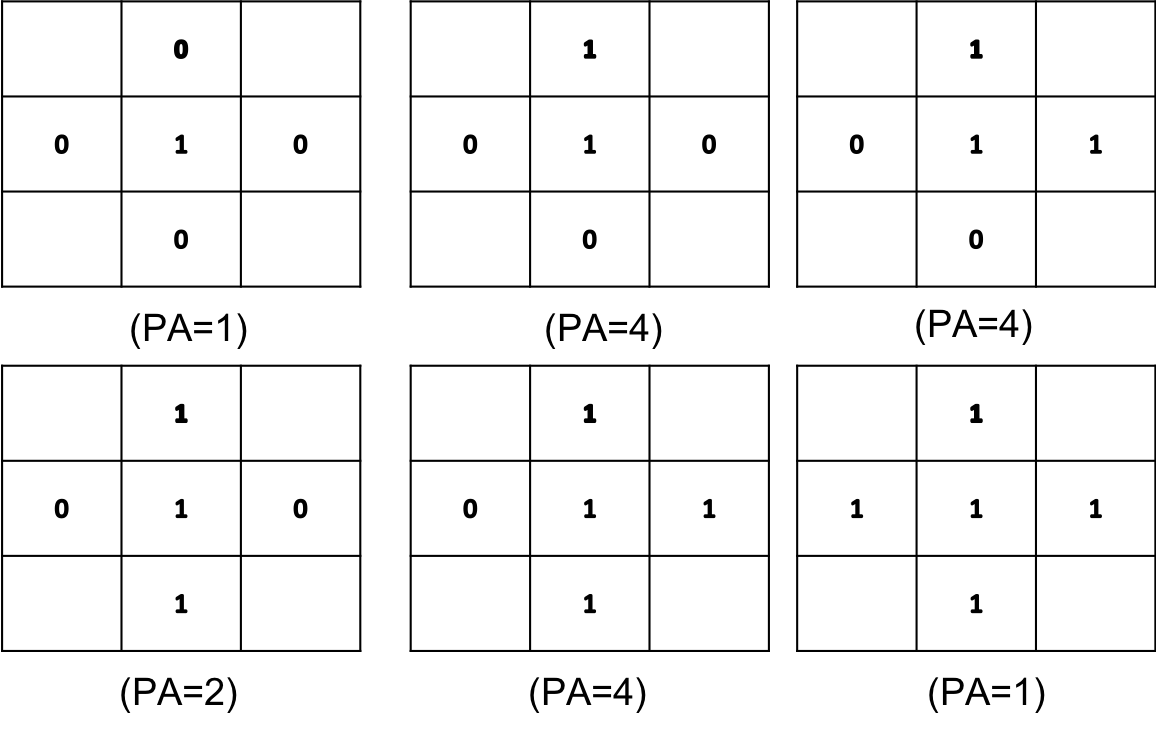
\includegraphics[width=\linewidth]{images/configuration.png}
	\caption{\textbf{Possible configuration states for micro-canonical ensemble.} There are total six possible configuration for energy calculation. Number 1 represents this neighbor is aligned with $\sigma_j$, number 0 represents this neighbor is not aligned with $\sigma_j$. PA represents the possible alignment for this configuration.}
	\label{fig:configuration}
\end{figure}
From the six possible configuration states, the Hamiltonian is obtained by summing up the spins of all four first neighbors, see fig \ref{fig:spins}. 
\begin{figure}
	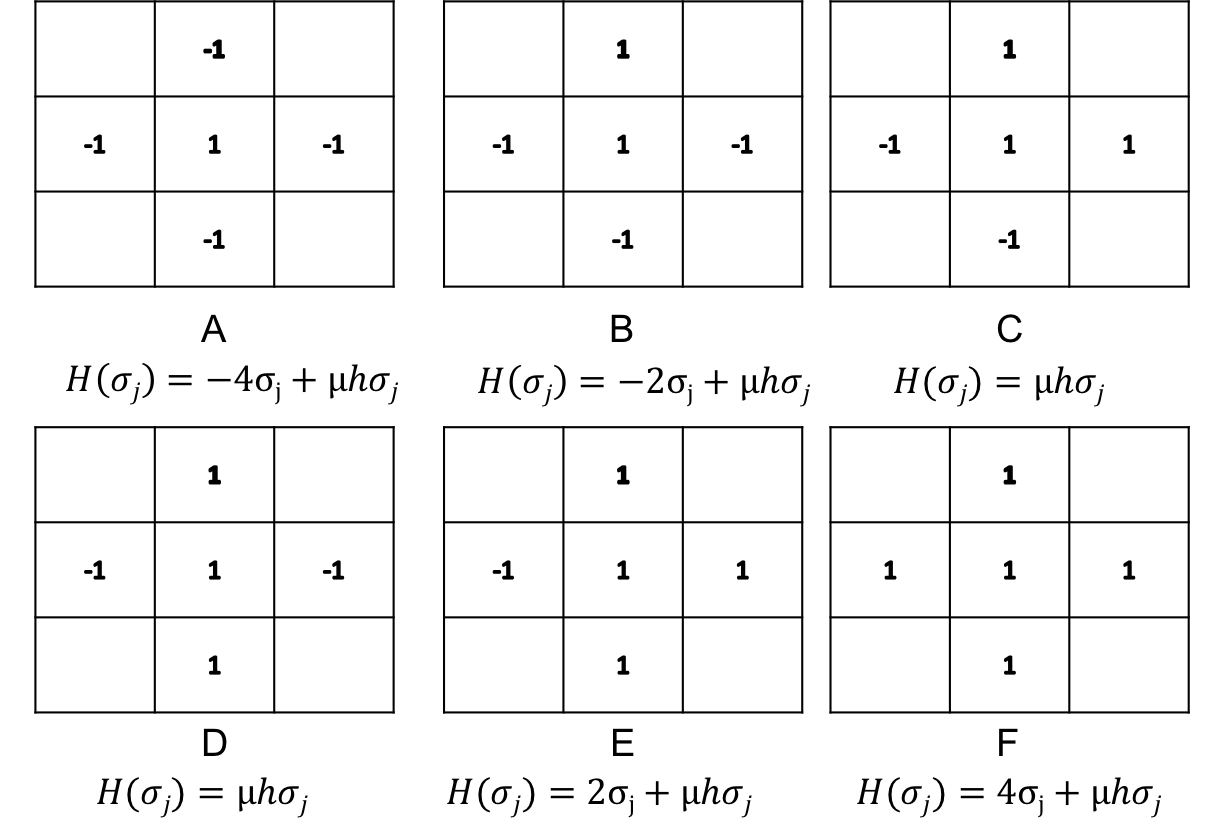
\includegraphics[width=\linewidth]{images/spins.png}
	\caption{\textbf{Spins for each possible configuration.} Considering the symmetry, a "mirror" state must be count for each configuration by flipping all five atoms at the same time, this gives the exact same configuration with the exact same energy. In this case, we can just divide by 2 for each configuration to get rid of the over-counting states.}
	\label{fig:spins}
\end{figure}
For each configuration, the partition function of micro canonical ensemble can be calculated using equation 2.1.2. By calculating the energy change by flipping $\sigma_j$ then we can assign Monte-Carlo moves to the system, and the probability is given in equation 2.1.3:
\begin{equation} 
\Lambda=e^{-\beta H} = e^{-\beta (\sum_{ij}  J\sigma_i\sigma_j+\sum_j\mu h\sigma_j) }
\end{equation}
Where $\beta=\frac{1}{k_BT}$, where $k_B$ is Boltzmann's constant and T is absolute temperature.
\begin{equation} 
P(\sigma_j)=\frac{1}{2} \frac{\Lambda(\sigma_j)}{\Lambda(-\sigma_j)}
\end{equation}
We randomly choose a number from zero to one to compare to $P(\sigma_j)$. If the number is smaller than $P(\sigma_j)$, then we accept the flip of the spin,otherwise, we reject the flip. In order to smooth the data, 10 different simulations with the same initial state but different initial configuration are accumulated and averaged. Different step size, temperature, and $\mu$ are assigned to carry out a comparative study.
For another approach,  the partition function of canonical ensemble is evaluated and further the probability for all possible configurations is calculated using equation 2.1.4 and 2.1.5:
\begin{equation} 
q(\sigma_j)=\sum_{\sigma_j} e^{-\beta H(\sigma_j)}
\end{equation}
\begin{equation} 
P=\frac{\Lambda}{q(\sigma_j)}=\frac{e^{-\beta H}}{\sum_{\sigma_j} e^{-\beta H(\sigma_j)}}
\end{equation}


\newpage
\section{Results/Discussion}

From Fig.~3, we can see that for small system sizes, the system can easily converge to a single spin state. However, for larger systems, convergence to a single spin state is much less likely. 

\begin{figure}[h!]
	\centering
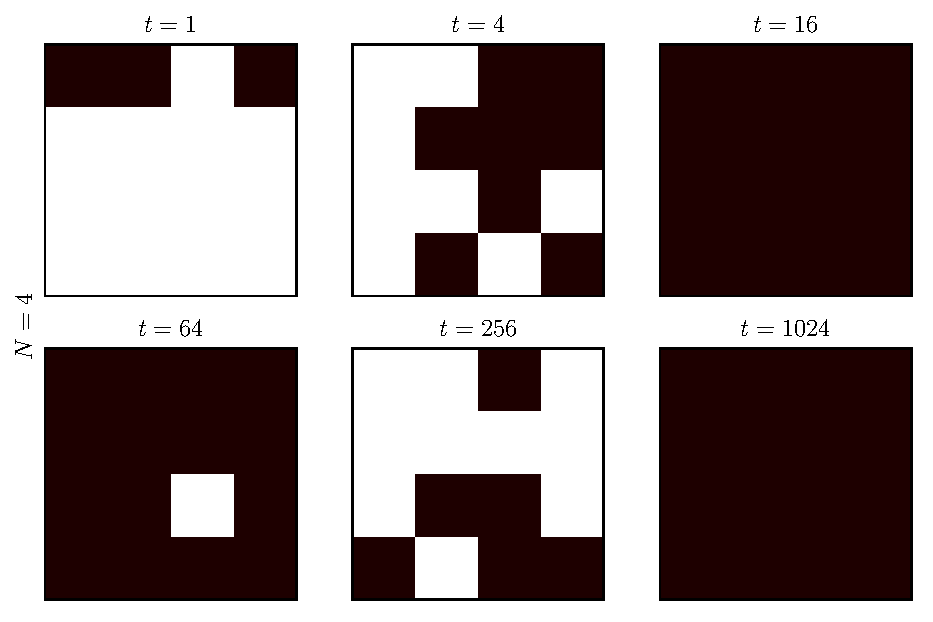
\includegraphics[scale=0.25]{images/image4_0_0.pdf}
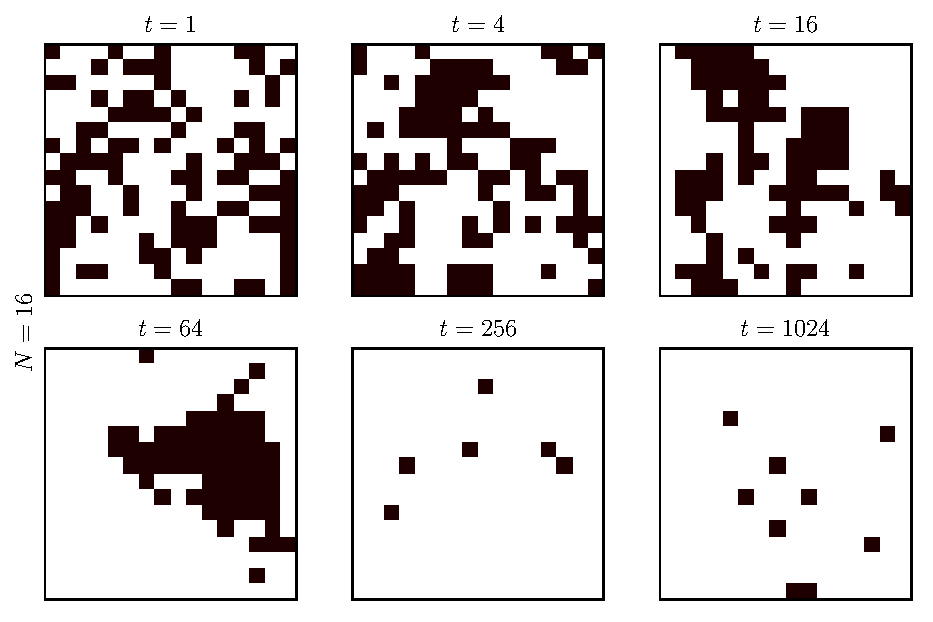
\includegraphics[scale=0.25]{images/image16_0_0.pdf}
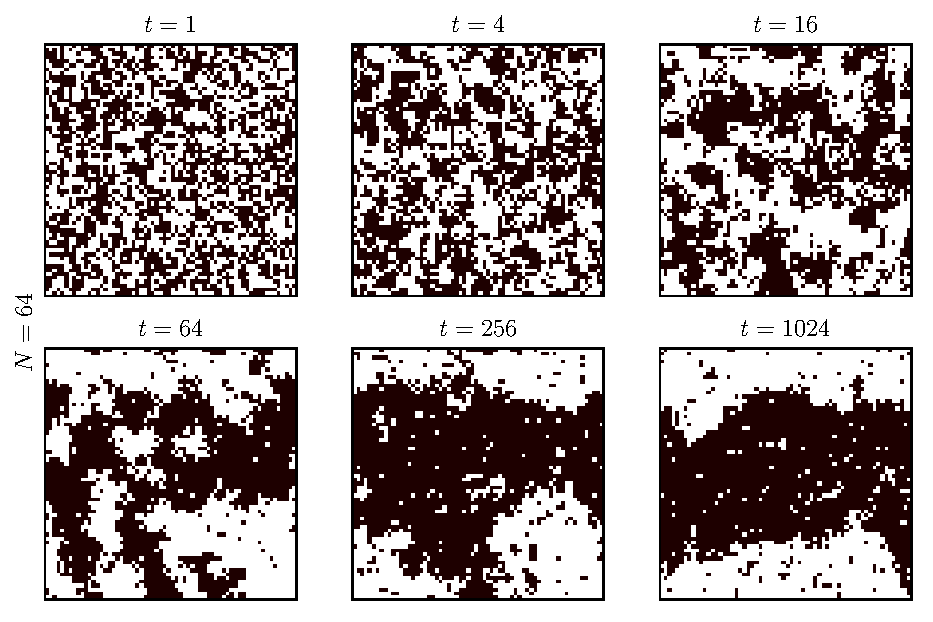
\includegraphics[scale=0.25]{images/image64_0_0.pdf}
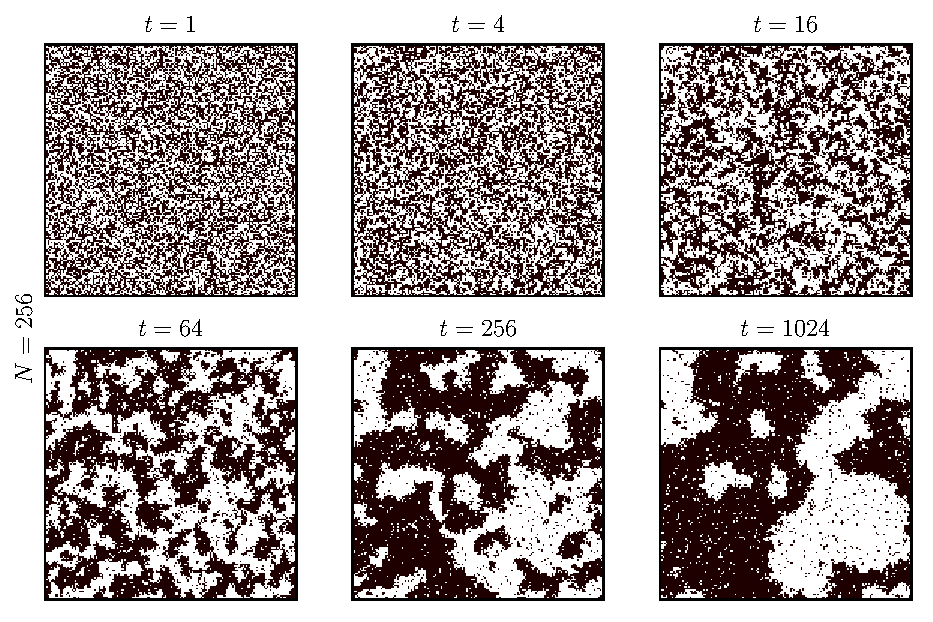
\includegraphics[scale=0.25]{images/image256_0_0.pdf}
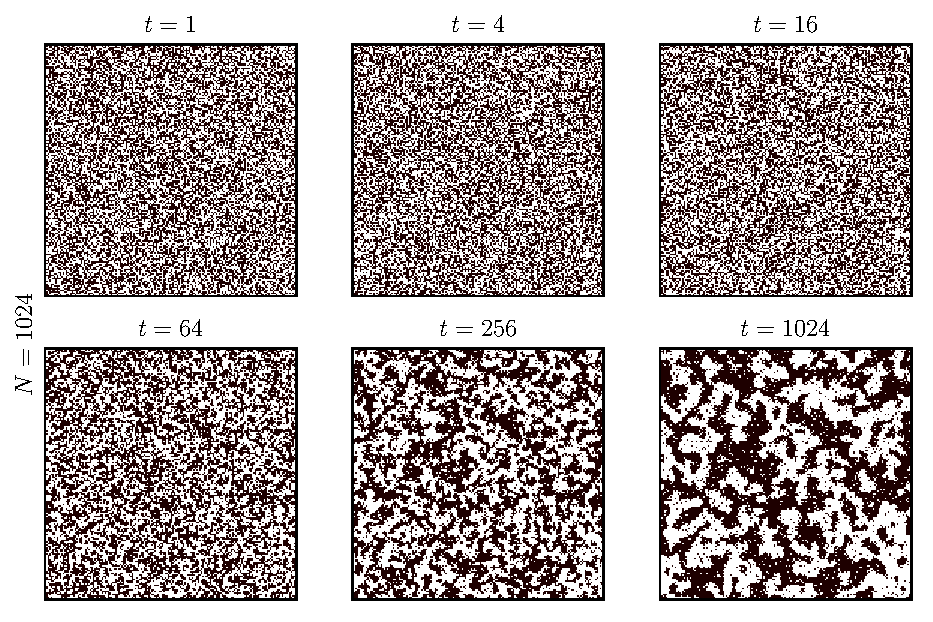
\includegraphics[scale=0.25]{images/image1024_0_0.pdf}
\caption{Evolution systems of various sizes for $\beta=0.5$,$\mu=0$.}
\end{figure}

From Fig.~4 we can see that in general, the average energy increases with temperature. Increasing $\tilde\mu$ serves to in decrease the temperature. 

\begin{figure}[h!]
	\centering
	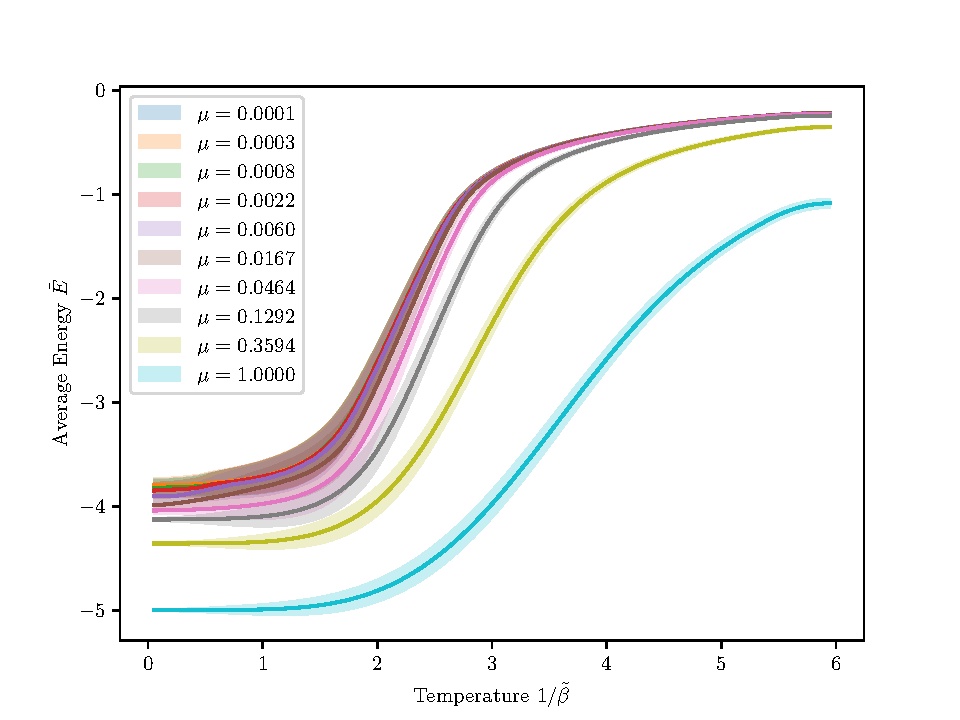
\includegraphics[scale=0.75]{images/energy.pdf}
	\caption{Average Energy vs. Temperature for various $\mu$.}
\end{figure}

Looking at Fig.~5 we can see that the magnetization increases with decreasing temperature, but the standard deviation of the magnetization for low temperatures is very large. 

\begin{figure}[h!]
	\centering
	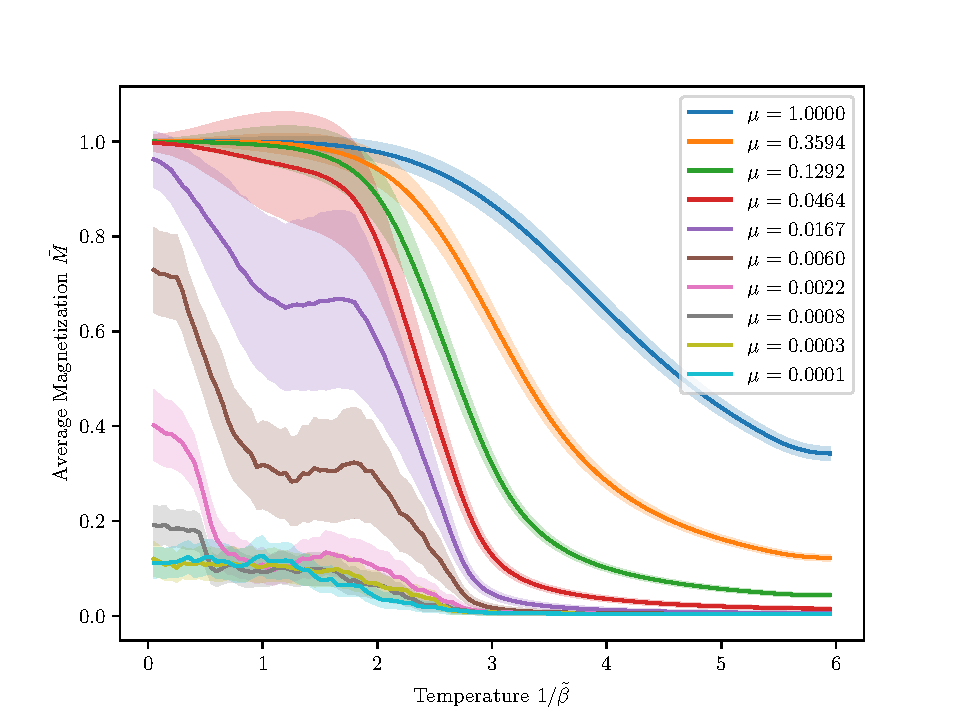
\includegraphics[scale=0.75]{images/magnet.pdf}
	\caption{Average Magnetization vs. Temperature for various $\mu$}
\end{figure}

In Fig.~6 we can see that regardless of the initial magnetization, the system evolves to a steady state depending on the temperature. One that is sensitive to magnetic fields and one that ether retains or spontaneously develops the magnetization. Below this critical temperature, the the material is ferromagnetic, above the temperature the system is paramagnetic. With no external field, we see that determine that the critical temperature is around $1/\tilde\beta= 2.5$. This value is consistent with \cite{onsager}. 

\begin{figure}[h!]
	\centering
	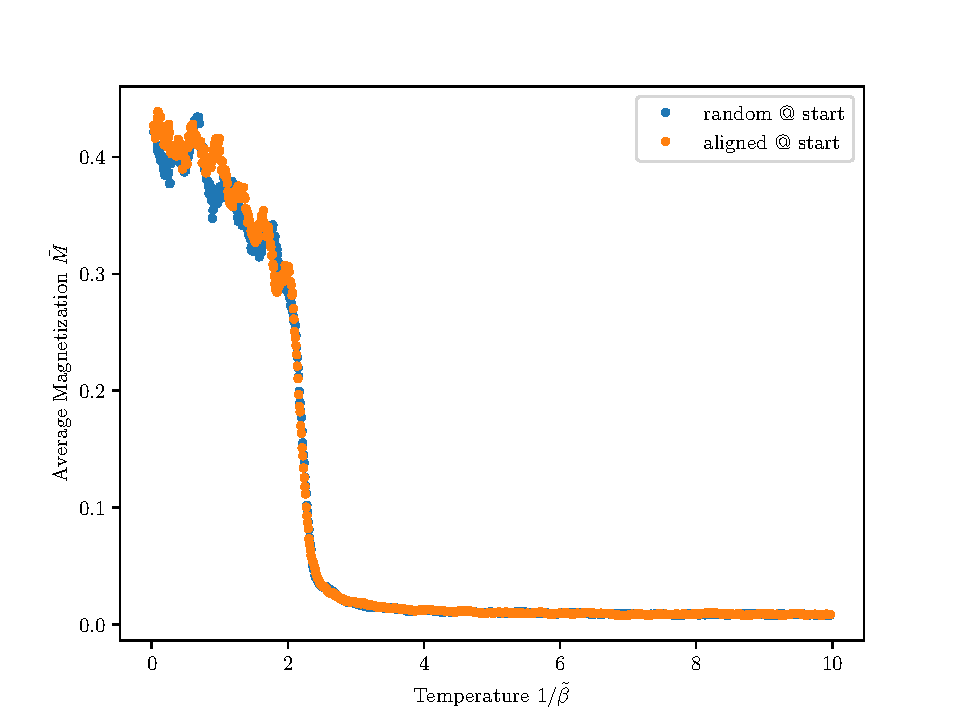
\includegraphics[scale=0.75]{images/ferropara.pdf}
	\caption{Magnetization at equilibrium for states starting off randomly and states starting off aligned. }
\end{figure}

 Fig.~7 shows a paramagnetic phase of $400\times400$ Ising model with a space-variable magnetic field. We see that as time increases, the local spins align with the local magnetic field.

\begin{figure}[h!]
	\centering
	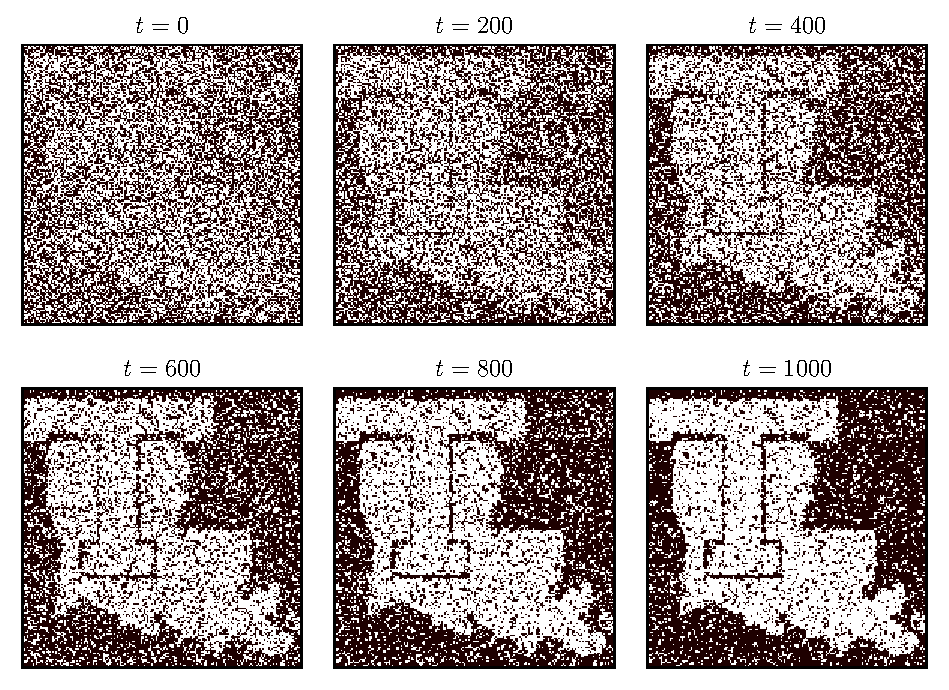
\includegraphics[scale=0.75]{images/latech.pdf}
	\caption{Ising model with space-variable magnetic field.}
\end{figure}



\section{Conclusion}
We conclude that the Ising model is a shows para/ferromagnetic phase transition at a critical temperature around $1/\tilde\beta= 2.5$. We see that the effect of the external magnetic field is to increase the energy and increase the magnetization. We also show that the spins can align to form an image when in the paramagnetic phase. 

%
% ---- Bibliography ----
%
\begin{thebibliography}{5}
%
\bibitem {onsager}
Onsager, Lars (1944), "Crystal statistics. I. A two-dimensional model with an order-disorder transition", Physical Review, Series II, 65 (3–4): 117–149,Bibcode:1944PhRv...65..117O, doi:10.1103/PhysRev.65.117, MR 0010315
\bibitem{rajeshrinet} https://rajeshrinet.github.io/blog/2014/ising-model/
\bibitem{weigel} https://arxiv.org/pdf/1006.3865.pdf
\bibitem{robert}https://arxiv.org/pdf/1504.01896.pdf
\end{thebibliography}

\end{document}
